\documentclass{standalone}
\usepackage{tikz}

\begin{document}
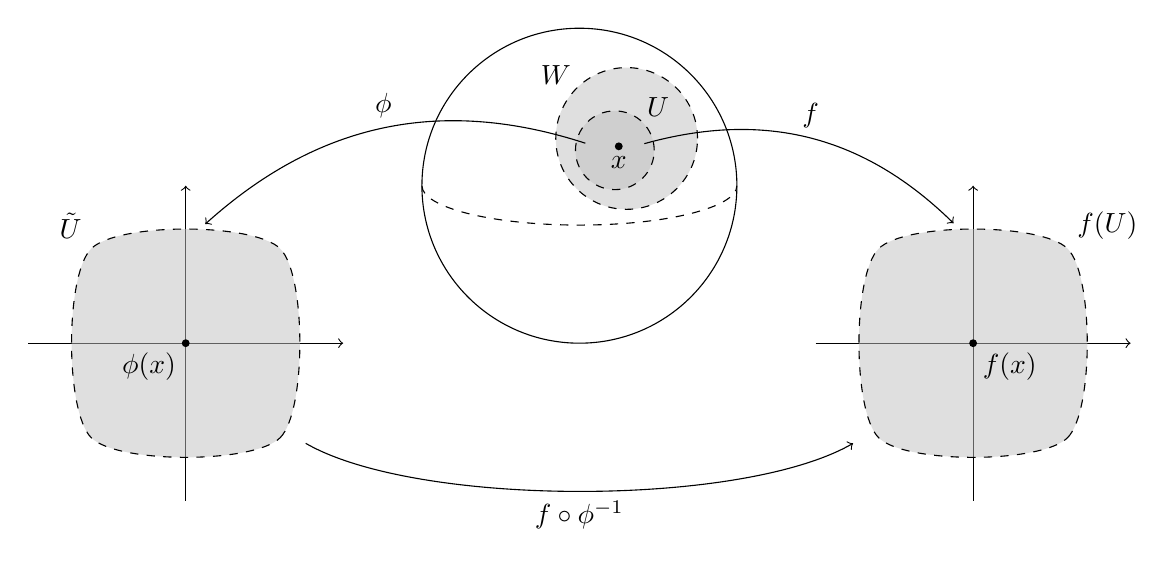
\begin{tikzpicture}
	\draw (0,0) circle[radius=2];
	\draw[dashed] (-2,0) arc[start angle=180, end angle=360, x radius=2, y
		radius=0.5];
  \filldraw[dashed, fill opacity=0.5, fill=gray!50] (0.6,0.6) circle (0.9);
  \node at (-0.3, 1.4) {$ W $};
  \filldraw[dashed, fill opacity=0.5, fill=gray!50] (0.45,0.45) circle (0.5);
  \node at (1,1) {$ U $ };
  \fill (0.5,0.5) circle (0.05);
  \node at (0.5,0.5) [below] {$ x $};
  \node (U1) at (0.2, 0.5) {};
  \node (U2) at (0.7, 0.5) {};

  \begin{scope}[xshift=5cm, yshift=-2cm]
    \draw[->] (-2,0) -- (2,0);
    \draw[->] (0,-2) -- (0,2);

    \filldraw[dashed, fill opacity = 0.5, fill = gray!50] plot[smooth cycle]
      coordinates{(-1.2,-1.2) (1.2,-1.2) (1.2,1.2) (-1.2,1.2)};

    \node[above right] at (1.2, 1.2) {$ f(U) $};
    \node (fU1) at (-1.4, -1.2) {};
    \node[left] (fU2) at (0,1.4) {};
    \fill (0,0) circle (0.05) node[below right]{$ f(x) $};
  \end{scope}
  
  \begin{scope}[xshift=-5cm, yshift=-2cm]
    \draw[->] (-2,0) -- (2,0);
    \draw[->] (0,-2) -- (0,2);

    \filldraw[dashed, fill opacity = 0.5, fill = gray!50] plot[smooth cycle]
      coordinates{(-1.2,-1.2) (1.2,-1.2) (1.2,1.2) (-1.2,1.2)};

    \node [above left] at (-1.2, 1.2) {$ \tilde{U} $};
    \node (Ut1) at (1.4, -1.2) {};
    \node[right] (Ut2) at (0, 1.4) {};
    \fill (0,0) circle (0.05) node[below left]{$ \phi(x) $};
  \end{scope}

  \draw[->, bend right] (U1) to node[above]{$ \phi $} (Ut2);
  \draw[->, bend right, looseness=0.6] (Ut1) to node[below]{$ f \circ \phi ^{-1} $} (fU1);
  \draw[<-, bend right] (fU2) to node[above]{$ f $} (U2);


\end{tikzpicture}
\end{document}
